\documentclass[a4paper, 12pt]{article}
\usepackage{amssymb}
\usepackage{amsmath}
\usepackage{verbatim}
\setcounter{tocdepth}{3}
\usepackage{graphicx}
\usepackage{afterpage}
\usepackage{floatpag}
\usepackage{setspace}
\floatpagestyle{empty}
%\usepackage[a4paper, total={4in, 6in},margin=4in]{geometry}
\usepackage[export]{adjustbox}
%\usepackage[paperwidth=7.0in, paperheight=10.7in]{geometry}
%\usepackage{layout}
%\layout{layoutwidth=180mm,layoutheight=227mm}
%\geometry{a4paper,left=25mm,right=25mm,top=25mm,bottom=25mm,heightrounded}
%\usepackage[a4paper]{geometry}
\usepackage{listings}
\usepackage{subfigure}
\usepackage{wrapfig}
\usepackage{float}
\usepackage[hyperindex=false,colorlinks=false]{hyperref}
\usepackage{fullpage}
\usepackage{tikz}
%\renewcommand{\floatpagefraction}{0.8}
%\renewcommand{\topfraction}{0.8}
\renewcommand{\bottomfraction}{0.8}
\usetikzlibrary{shapes.geometric, arrows}
\DeclareMathSizes{20}{20}{20}{20}

\tikzstyle{startstop}=[rectangle, rounded corners, minimum width=3cm, minimum height=1cm, text centered, text width=4cm, draw=black,fill=red!30]

\tikzstyle{io}=[trapezium, trapezium left angle=70, trapezium right angle=110, minimum width=3cm, minimum height=1cm, text centered, text width=4cm, draw=black, fill=blue!30]

\tikzstyle{process}=[rectangle, minimum width=3cm, minimum height=1cm, text centered, text width=4cm, draw=black,fill=orange!30]

\tikzstyle{decision}=[diamond, minimum width=3cm, minimum height=1cm, text centered, text width=4cm, draw=black, fill=green!30]

\tikzstyle{arrow}=[thick,->,>=stealth]

\begin{document}

\begin{titlepage}

%\newcommand{\HRule}{\rule{\linewidth}{0.5mm}} % Defines a new command for the horizontal lines, change thickness here
\newcommand{\HRule}{\rule{155mm}{0.5mm}} % Defines a new command for the horizontal lines, change thickness here

\center % Center everything on the page

%----------------------------------------------------------------------------------------
%   HEADING SECTIONS
%----------------------------------------------------------------------------------------

\textsc{\LARGE Technische Universit{\"a}t M{\"u}nchen}\\[1.5cm] % Name of your university/college
\textsc{\Large Chair For Computer Technology and Computer Organisation}\\[0.5cm] % Major heading such as course name

%----------------------------------------------------------------------------------------
%   TITLE SECTION
%----------------------------------------------------------------------------------------
\vspace{30mm}
\begin{center}
\Large\textit{Guided Research}
\end{center}
\HRule \\[0.4cm]
{ \Large \bfseries A Protocol for the Integration of Invasive Resource Management into Standard Batch Schedulers}\\[0.5cm] % Title of your document
\HRule \\[1.5cm]

%----------------------------------------------------------------------------------------
%   AUTHOR SECTION
%----------------------------------------------------------------------------------------
\vspace{48mm}
\begin{minipage}{0.4\textwidth}
\begin{flushleft} \large
\emph{Student:}\\
Nishanth Nagendra % Your name
\end{flushleft}
\end{minipage}
\begin{minipage}{0.4\textwidth} 
\begin{flushright} \large
\emph{Supervisor:} \\
Prof. Dr. Michael Gerndt \\~\\ % Supervisor's Name
\emph{Advisor:} \\
M.Sc. Isaias Alberto Compres Urena  % Advisor's Name
\end{flushright}
\end{minipage}\\[2cm]

% If you don't want a supervisor, uncomment the two lines below and remove the section above
%\Large \emph{Author:}\\
%John \textsc{Smith}\\[3cm] % Your name

%----------------------------------------------------------------------------------------
%   DATE SECTION
%----------------------------------------------------------------------------------------

{\large \today}\\[2cm] % Date, change the \today to a set date if you want to be precise

\end{titlepage}

\begin{center}
\huge \bfseries Acknowledgement
\end{center}
\thispagestyle{empty}
\vspace{35mm}
I would like to thank  Isaias for his constant support and guidance throughout the guided research especially when I faced some challenges in understanding certain topics. I would also like to thank Prof. Dr. Michael Gerndt for providing me with this opportunity to work on such an interesting topic.

\newpage

\begin{center}
\huge \bfseries Abstract
\end{center}
\thispagestyle{empty}
\vspace{35mm}
\noindent
Invasive computing is a novel paradigm for the design and resource-aware programming of future parallel computing systems. It enables the programmer to write resource aware programs and the goal is to optimize the program for the available resources. Traditionally, parallel applications implemented using MPI are executed with a fixed number of MPI processes while submitting to a HPC(High Performance Computing) center. This results in a fixed allocation of resources for the job. Newer techniques in scientific computing such as AMR(Adaptive mesh refinement) result in applications exhibiting complex behavior where their resource requirements change during execution. Invasive MPI which is a part of an ongoing research effort to provide MPI extensions for the development of Invasive MPI applications will result in evolving jobs at runtime supporting such AMR techniques in HPC centers. Unfortunately, using only static allocations result in the evolving applications being forced to execute using their maximum resource requirements that may lead to an inefficient resource utilisation. In order to support such parallel evolving applications at HPC centers, there is an urgent need to investigate and implement extensions to existing resource management systems or develop an entirely new one. These supporting infrastructures must be able to not only handle the evolving jobs but also the legacy rigid/static jobs intelligently and hence newer protocols for integration of such invasive resource management into existing standard batch systems needs to be now explored.

\newpage
\thispagestyle{empty}
\tableofcontents
\newpage
\listoffigures
\newpage

\setcounter{page}{1}
\section{Introduction}
Invasive computing is a novel paradigm for the design and resource-aware programming of future parallel computing systems. It enables the programmer to write efficient resource aware programs. This approach can be used to allocate, execute on and free resources during execution of the program. HPC infrastructure like Clusters, Supercomputers execute a vast variety of jobs, majority of which are parallel applications. These centers use intelligent resource management systems that should not only perform tasks of job management, resource management and scheduling but also satisfy important metrics like higher system utilization, job throughput and responsiveness. Traditionally, MPI applications are executed with a fixed number of MPI processes but with Invasive MPI they can evolve dynamically at runtime in the number of their MPI processes. This in turn supports advanced techniques like AMR where the working set size of applications change at runtime. These advancements entail an immediate need for stronger and intelligent resource management systems that can provide efficient resource utilization at HPC centers. They should also now be able to achieve much higher system utilisation, energy efficiency etc. compared to their predecessors due to elasticity of the applications.\par
\noindent
\\Under the collaborative research project funded by the German research foundation(DFG) in the Transregional Collaborative Research Centre 89(TRR89), research efforts are being made to investigate Invasive computing approach at different levels of abstraction vertically right from the hardware up to the programming model. Invasive MPI is one such effort towards invasive programming with MPI where the application programmer has MPI extensions available using which he/she can specify at certain safe points in the program, triggers that allow for elasticity which means the application can evolve.

\subsection{Resource Management}
In order to support such parallel evolving applications at HPC centers there is an urgent need to investigate and implement extensions to existing resource management systems or develop an entirely new one. These supporting infrastructures must be able to handle the new kind of evolving jobs/applications and the legacy rigid jobs intelligently keeping in mind that they should now be able to achieve much higher system utilisation, energy efficiency etc compared to their predecessors due to the elasticity of the applications. Two of the most widely used resource managers on HPC systems are SLURM and TORQUE. A resource manager together with a batch scheduler forms what is called as a Batch System that is complex piece of middleware used for managing supercomputing resources. 
\subsection{Batch Scheduling}
The batch scheduler accepts job descriptions given by end users some of which mention as to how long the job would run and the amount of resources it will need. It maintains a queue of jobs and dispatches them to the process manager based on some criteria and algorithms. The decisions made depend on the state of resources and also others like job priorities, fairness, waiting times etc. The process manager on the other hand has lesser intelligence and does the task of mapping the processes of a parallel application on the hardware based on the node list provided to it by the batch scheduler. In the context of invasive computing we need to be investigate for new requirements in the interaction between the batch scheduler and process manager. The decisions made by the batch scheduler need to be influenced to support evolving jobs.\par
\noindent
\\In contrast to the earlier uni-directional communication from batch scheduler to process manager, we now need to support a bi-directional communication between the two. The capabilities of existing batch schedulers could be leveraged rather than having to replace an entire system with a new one. The possibility of supporting a new interface for the existing batch scheduler needs to be explored such that it communicates with a new invasive process management that controls a dedicated partition to support invasive computing. An investigation needs to be done on whether the existing interface of batch schedulers towards process manager could be extended or re-used and also on the possiblity of receiving feedback from the invasive process manager to allow the batch scheduler to be influenced. The invasive process manager one level below in the hierarchy will work on local metrics of the dedicated invasive partition within the cluster. In addition to this it will also perform some kind of a run time scheduling for pinning the jobs to the nodes in the partition and also run time tuning of the parallel applications. Due to this it is more than just being a process manager and will therefore be referred to as Invasive Resource Manager.\par
\noindent
\\The investigations of this guided research are an initial study that will support the continuing research effort for developing Invasive MPI and extended resource management systems to support invasive computing.

\newpage
\section{Invasive Computing}
The throughput of supercomputers depend not only on efficient job scheduling but also on the type of jobs that form the workload. Malleable jobs are most favourable for a cluster as they can dynamically adapt to a changing allocation of resources. The batch system can expand or shrink a running malleable job to improve system utilization, throughput, and response times. In the past, however the rigid nature of commonly used programming models like MPI made writing malleable applications a daunting task, which is why it remains largely unrealized. This is now changing. To improve fault tolerance, load imbalance, and energy efficiency in emerging exascale systems more adaptive programming paradigms are being investigated. Although they may offer better support for malleability, current batch systems still lack management facilities for malleable jobs and are therefore incapable of leveraging their potential. In this guided research we propose an extension to the SLURM resource manager to support malleable jobs.
\subsection{Job Classification}
As defined by Feitelson and Rudolph [1], jobs can be classified into four categories based on their flexibility.
\begin{itemize}
\item \textbf{\textit{Rigid job:}} This is the most common type which requires a fixed number of processors throughout its execution.
\item \textbf{\textit{Moldable job:}} In this kind of job the resource set can be molded or modified by the batch system before starting the job (e.g. to effectively fit alongside other rigid jobs). Once started its resource set cannot be changed anymore.
\item \textbf{\textit{Evolving job:}} These kind of jobs request for resource expansion or shrinkage during their execution. Applications that use multiscale analysis like Quadflow or Adaptive mesh refinement(AMR) exhibit this kind of behavior typically due to unexpected increases in computations or having reached hardware limits(e.g. memory) on a node. 
\item \textbf{\textit{Malleable job:}} The expansion and shrinkage of resources are initiated by the batch system in contrast to the evolving jobs. The application adapts itself to the changing resource set.
\end{itemize}
The first two types fall into the category of what is called as the static allocation since the allocation of rigid and moldable jobs must be finalized before the job starts. Whereas, the last two types fall under the category of dynamic allocation since this property of expanding or shrinking evolving and malleable jobs(together termed adaptive jobs) happens at runtime.\par
\noindent
\\
Malleable jobs hold a strong potential to obtain high system performance. Batch systems can substantially improve the system utilization, throughput and response times with efficient shrink/expand strategies for malleable jobs. Similarly, applications also profit when expanded with additional resources as this can increase application speedup and improve load balance across the job’s resource set. Enabling malleable jobs in cluster systems requires three major components: (i) a parallel runtime that is able to adapt to a changing resource set, (ii) a batch system with dynamic allocation facilities, and (iii) a communication mechanism between the two. Traditionally, all batch systems support only static allocations.\par

\subsection{Traditional Resource Management}
The role of a resource manager is that it acts like a \textit{glue} for a parallel computer to execute parallel jobs. It should make a parallel computer as easy to use as almost a PC. MPI would typically be used to manage communications within the parallel program. A resource manager allocates resources within a cluster, launches and otherwise manages jobs. Some of the examples of widely used open source as well as commercial resource managers are \textbf{SLURM, TORQUE, OMEGA, IBM Platform LSF} etc. Together with a scheduler it is termed as a \textbf{\textit{Batch System}}. The Batch System serves as a middleware for managing supercomputing resources. The combination of \textit{Scheduler}$+$\textit{Resource Manager} makes it possible to run parallel jobs.\par
\noindent
\\
The role of a job scheduler is to manage queue(s) of work when there is more work than resources. It supports complex scheduling algorithms which are optimized for network topology, energy efficiency, fair share scheduling, advanced reservations, preemption, gang scheduling(time-slicing jobs) etc. It also supports resource limits(by queue, user, group, etc.). Many batch systems provide both resource management and job scheduling within a single product (e.g. LSF) while others use distinct products(e.g. Torque resource manager and Moab job scheduler). Some other examples of Job scheduling systems are \textbf{LoadLeveler, OAR, Maui, SLURM} etc.\par
\noindent
\\
The prime focus of this work will be on SLURM(Simple Linux Utility For Resource Management) which will be the choice of batch system upon which the support for Invasive Computing will be demonstrated. SLURM is a sophisticated open source batch system with about 500,000 lines of C code whose development started in the year 2002 at Lawrence Livermore National Laboratory as a simple resource manager for Linux Clusters and a few years ago spawned into an independent firm under the name SchedMD. SLURM has since its inception also evolved into a very capable job scheduler through the use of optional plugins. It is used on many of the world's largest supercomputers and is used by a large fraction of the world's TOP500 Supercomputer list. It supports many UNIX falvors like AIX, Linux, Solaris and is also fault tolerant, highly scalable, and portable.\par
\noindent
\\
Plugins are dynamically linked objects loaded at run time based upon configuration file and/or user options. Approximately $80$ plugins of different varities are currently available. Some of them are listed below:\\
\begin{itemize}
\item \textbf{\textit{Accounting storage:}} MySQL, PostgreSQL, textfile.
\item \textbf{\textit{Network Topology:}} 3D-Torus, tree.
\item \textbf{\textit{MPI:}} OpenMPI, MPICH1, MVAPICH, MPICH2, etc.
\end{itemize} 
PLugins are typically loaded when the daemon or command starts and persist indefinitely. They provide a level of indirection to a configurable underlying function.
\begin{figure}[h]
\centering
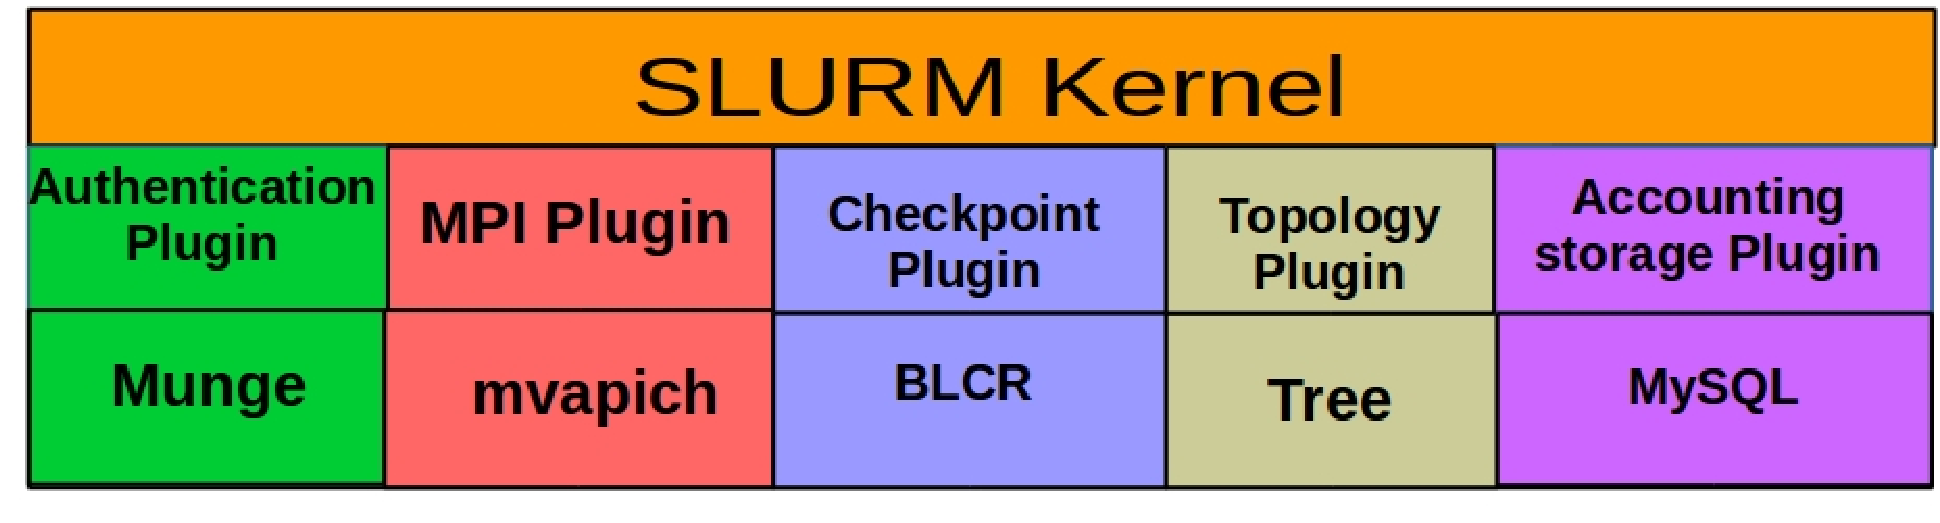
\includegraphics[width=1.0\textwidth]{./plugin.eps}
\vspace{-0.15in}
\caption{Software layers of SLURM}
\label{fig:6}
\end{figure}
\subsection{Support For Invasive Computing}
Existing batch systems usually only support static allocation of resources to applications before job start. Hence we need some kind of an Invasive Resource Management to be integrated into these existing batch systems so that we can support malleable jobs allowing us to change the allocated resources dynamically at runtime. In order to achieve this we will follow the below approach:
\begin{itemize}
\item \textbf{\textit{Invasive Resource Manager (alias iHypervisor):}} An independent component which will talk to the current batch systems via a communication mechanism(protocol) to obtain invasive job(s) submitted specifically to the invasic partition that can support invasive computing. The iHypervisor will then take these jobs and perform some kind of runtime scheduling for pinning these jobs to the resources in the partition and makes these decisions in order to optimize certain local metrics such as resource utilization, power stability, energy efficiency etc. The scheduling here is done at the granularity of cores and sockets. iHypervisor is the one that has the complete information of the resources in the invasic partition and also manages them. This component in an independent entity with the purpose of inter-operating with existing batch systems rather than replacing them with an entirely new one. It may be possible that in the future this component will not be a separate entitiy but will be built into the batch system itself.
\item \textbf{\textit{Invasive Job Scheduler (alias iScheduler):}} This component will be a new extension built into the existing batch systems for performing job scheduling. The scheduling decisions are communicated via the protocol used to speak to iHypervisor and these decisions are basically job(s) selected via a scheduling algorithm to be submitted to the iHypervisor for execution. The scheduling decisions will be made on the basis of available resources in the partition and it is the iHypervisor that communicates this to iScheduler in the form of resource offers (Real/Virtual). It can be a virtual resource offer because the iHypervisor can hide the real resources and present a rather fake view of them to iScheduler in the hope of getting a mapping of jobs to offer that is more suitable to satisfy its local metrics. Similar to iHypervisor, the iScheduler makes its decisions to optimize for certain local metrics such as high job throughput, reduced job waiting times, deadlines, priorities etc. This highlights the mismatching policies/metrics for which both the iHypervisor and iScheduler make their decisions on and hence both will be involved in some kind of a negotiation via the protocol to reach a common agreement.
\item \textbf{\textit{Negotiation Protocol:}} This protocol forms the core of the interaction between the iScheduler and iHypervisor. It allows for iHypervisor to make one or a set of resource offers to iScheduler which then needs to select jobs from its job queue to be mapped to these resource offers and finally sent back to the iHypervisor. The iHypervisor will then decide whether to accept/reject this mapping to satisfy its local metrics. If it accepts it will launch them based on some run time scheduling and if it rejects then it informs this to iScheduler in addition to sending it a new resource offer. The iScheduler can also reject the resource offers in which case it will be sent a new one. On accepting an offer, the iScheduler then repeats its tasks to send back a mapping to iHypervisor and this interaction continues until both reach a common agreement. If the number of such attempts reach a threshold then iScheduler will just accept whatever offer it receives and iHypervisor will also accept whatever Map:Jobs$\rightarrow$Offers it receives closing this transaction of negotiating. After this a new transaction will start.
\item \textbf{\textit{SLURM:}} SLURM is our choice of an existing batch system upon which this new implementation will be demonstrated as a proof of concept to support the new paradigm of resource-aware programming in the domain of invasive computing.
\end{itemize}
\noindent
This project implements a testing prototype for demonstrating how such an approach to support invasive computing with the above entities may work. It will involve implementing the communication infrastructure using SLURM API due to which iHypervisor and iScheduler will interact with each other using protocol messages filled with dummy values. It will also involve implementing the iScheduler as a new plugin(multithreaded) for SLURM and iHypervisor as a fake multithreaded Invasive Resource Manager daemon with bare minimum functionalities that in the near future will be an enhanced version of the daemon slurmd(built on top of it) found in SLURM. For the purposes of testing this prototype, the different scenarios that can be observed most of the time with the kind of negotiation protocol described earlier would be verified.
%\noindent
\clearpage
\section{Design and Implementation}
This section illustrates and describes a high level design of the software implemented with the help of protocol sequence diagrams and state machine diagrams. It will help to understand at a high level as to how the system has been designed to support this new approach of invasive computing and how will many of its components in the software hierarchy interact with each other with new protocols or extensions of existing protocols to integrate such an invasive resource management into current batch systems.
\subsection{Software Architecture}
The following page shows the software architecture of how Invasive Resource Management can be supported with a traditional resource manager and how exactly the new software components will fit in the existing software hierarchy. The figure [X] relates closely to how SLURM is organized since the intention of this work would be to demonstrate the support for Invasive Computing with the help of SLURM as a resource manager.
\begin{itemize}
\item The top layer is that of the core resource management component which has access to job queues. In this architecture, it will now have access to not only the queue for the legacy(static) jobs but also invasive job queue(jobs submittted to invasic partition that supports invasive computing).
\item In a traditional setup the top layer will perform the task of job scheduling as well. This means that it will select a job(s) from the queue of jobs based on the current state of resources and many other factors to dispatch it to the traditional process manager below in the hierarchy. The process manager then takes the responsibility of launching these jobs on the allocated resources in the partition and managing them for their full lifetime. In case of parallel jobs, it will manage the job in a parallel environment along with facilitating the communication amongst the parallel tasks/processes with the help of a PMI(Process Manager Interface) server. The process manager may also spawn slave daemons on each of the nodes which are a part of the resource allocation for a single job to manage them more effectively.
\item As discussed in the previous chapter, an independent Invasive resource management component by the name "iHypervisor" will be implemented which needs to communicate with a new scheduling component iScheduler and influence the scheduling decisions taken by it. The iHypervisor sits between the top layer and the process manager.
\item A new job scheduler specifically for invasive jobs needs to be integrated into the existing batch system. This is due to the reason that the scheduler for invasive jobs will work in a different manner based on the approach described earlier in comparison to the legacy job scheduler for static jobs. In case of SLURM which has a modular design with several optional plugins, a new plugin by name "iScheduler" will be implemented for SLURM to handle job scheduling specifically for invasic jobs.
\item Communication between iHypervisor and iScheduler will involve the negotiation protocol as explained in the previous chapter but will also include periodic feedbacks being sent by iHypervisor to iScheduler having some useful statistical measures about current state of resources, resource utilization, job throughput etc. that may help influence the decision making of iScheduler. This communication will also additionally support a means to service urgent jobs immediately.
\end{itemize}
\begin{figure}[!htbp]
\centering
\includegraphics[width=1.0\textwidth, height=185mm]{"software architecture".eps}
\caption{Invasive Resource Management Architecture}
\label{fig:7}
\end{figure}
\begin{figure}[h]
\centering
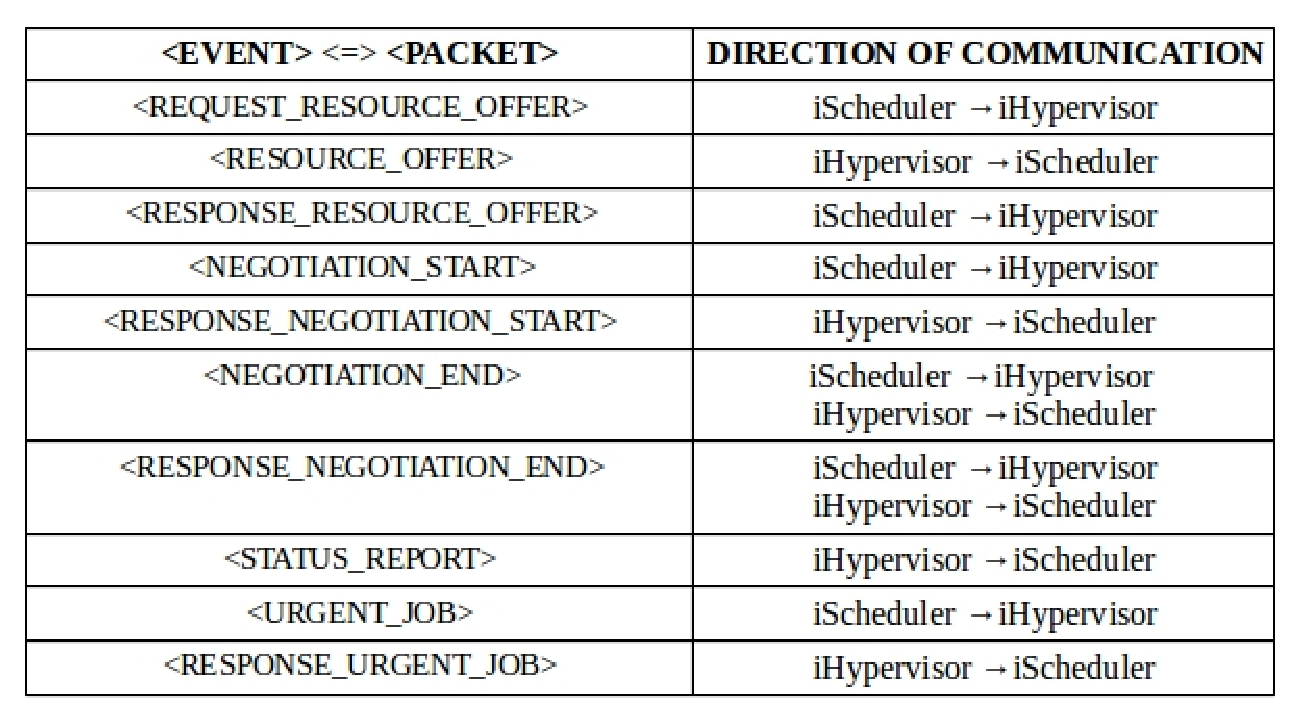
\includegraphics[width=1.0\textwidth, height=80mm]{table.eps}
\caption{Message Types}
\label{fig:8}
\end{figure}
%\begin{minipage}[t]
%\vspace{0mm}
%\afterpage{
%\begin{figure}[htbp]
%\floatpagestyle{empty}
%\hspace*{-0.3in}
%\raisebox{12mm}{
%\includegraphics[scale=0.95]{./diagram.eps}%}
%\caption{\textbf{Flow chart of the software imlementation}}
%\label{fig 1}
%\end{figure}
%}
%\end{minipage}[t]
%\afterpage%{
%\thispagestyle{empty}
%\begin{figure}[htbp]
%\floatpagestyle{empty}
%\hspace*{0.1in}
%\includegraphics[scale=0.9]{./diagram1.eps}
%\caption{\textbf{Pseudo code for algorithms}}
%\label{fig 2}
%\end{figure}
%}
%\afterpage{
%\thispagestyle{empty}
%\begin{figure}[htbp]
%\floatpagestyle{empty}
%\hspace*{-0.10in}
%\includegraphics[scale=0.85]{./diagram2.eps}
%\caption{\textbf{Pseudo code for algorithms}}
%\label{fig 3}
%\end{figure}
%}
\subsection{Communication Phases}
\begin{itemize}
\item \textbf{\textit{Protocol Initialization:}} This phase basically establishes the initial environment between the communicating parties (iScheduler and iHypervisor) for proper communication later on. Successful initialization of this phase prepares both the parties to start negotiating based on the negotiation protocol described in the following points. During this protocol initialization various parameters such as protocl version, maximum attempts for negotiation, timer intervals and several others could be exchanged to set up the internal data structures and configuration tables for both the communicating parties. This protocol is a bi-directional communication.
\item \textbf{\textit{Protocol Finalization:}} This phases signals the end of communication between iHypervisor and iScheduler using negotiation protocol. It leads to a safe termination of this communication followed by the release of any internal data structures allocated earlier along with configuration parameters. This results in consistent behaviour of both the communicating parties which can then proceed to safely terminate and exit. This protocol is a bi-directional communication.
\item \textbf{\textit{Negotiation:}} This is the most important phase in this whole approach to support invasive computing as discussed in the previous chapter. It is the phase during which both iHypervisor and iScheduler are negotiating with each other till they reach an agreement. If they do not then they continue till a certain limit to the number of negotiating attempts are reached after which both of them just agree in their final attempt closing the current negotiation. After this a new transaction of negotiation begins.
\item \textbf{\textit{Feedback:}} This concerns the periodic feedback sent by the iHypervisor to the iScheduler containing useful information such as the job states, latest snapshot of the resources in the invasic partition and many other statistical measures not limited to system utilization, job throughput, waiting times of jobs to help and influence the iScheduler in its decision making for scheduling jobs during its future transactions of negotiation. This protocol is a uni-directional communication.
\item \textbf{\textit{Urgent Jobs:}} This protocol concerns the support for urgent jobs. At any given point of time a cluster or supercomputing center may want to support very high priority jobs immediately without any further delay. By introducing support for invasive computing, it makes it all the more feasible to help run these urgent jobs immediately by either shrinking the resources of other jobs or suspending/Killing them.
\end{itemize}
\noindent
The following pages illustrate some sequence diagrams of how the negotiation protocol works with some of the important scenarios that will be encountered most of the time during the operation of the system. The sequence diagrams of other protocols are not shown in this document since they are simple and commonly observed type of protocols.
\clearpage
\subsection{Protocol Sequence Diagrams}
\vspace{-0.15in}
\begin{figure}[!htbp]
%\begin{figure}[H]
\centering
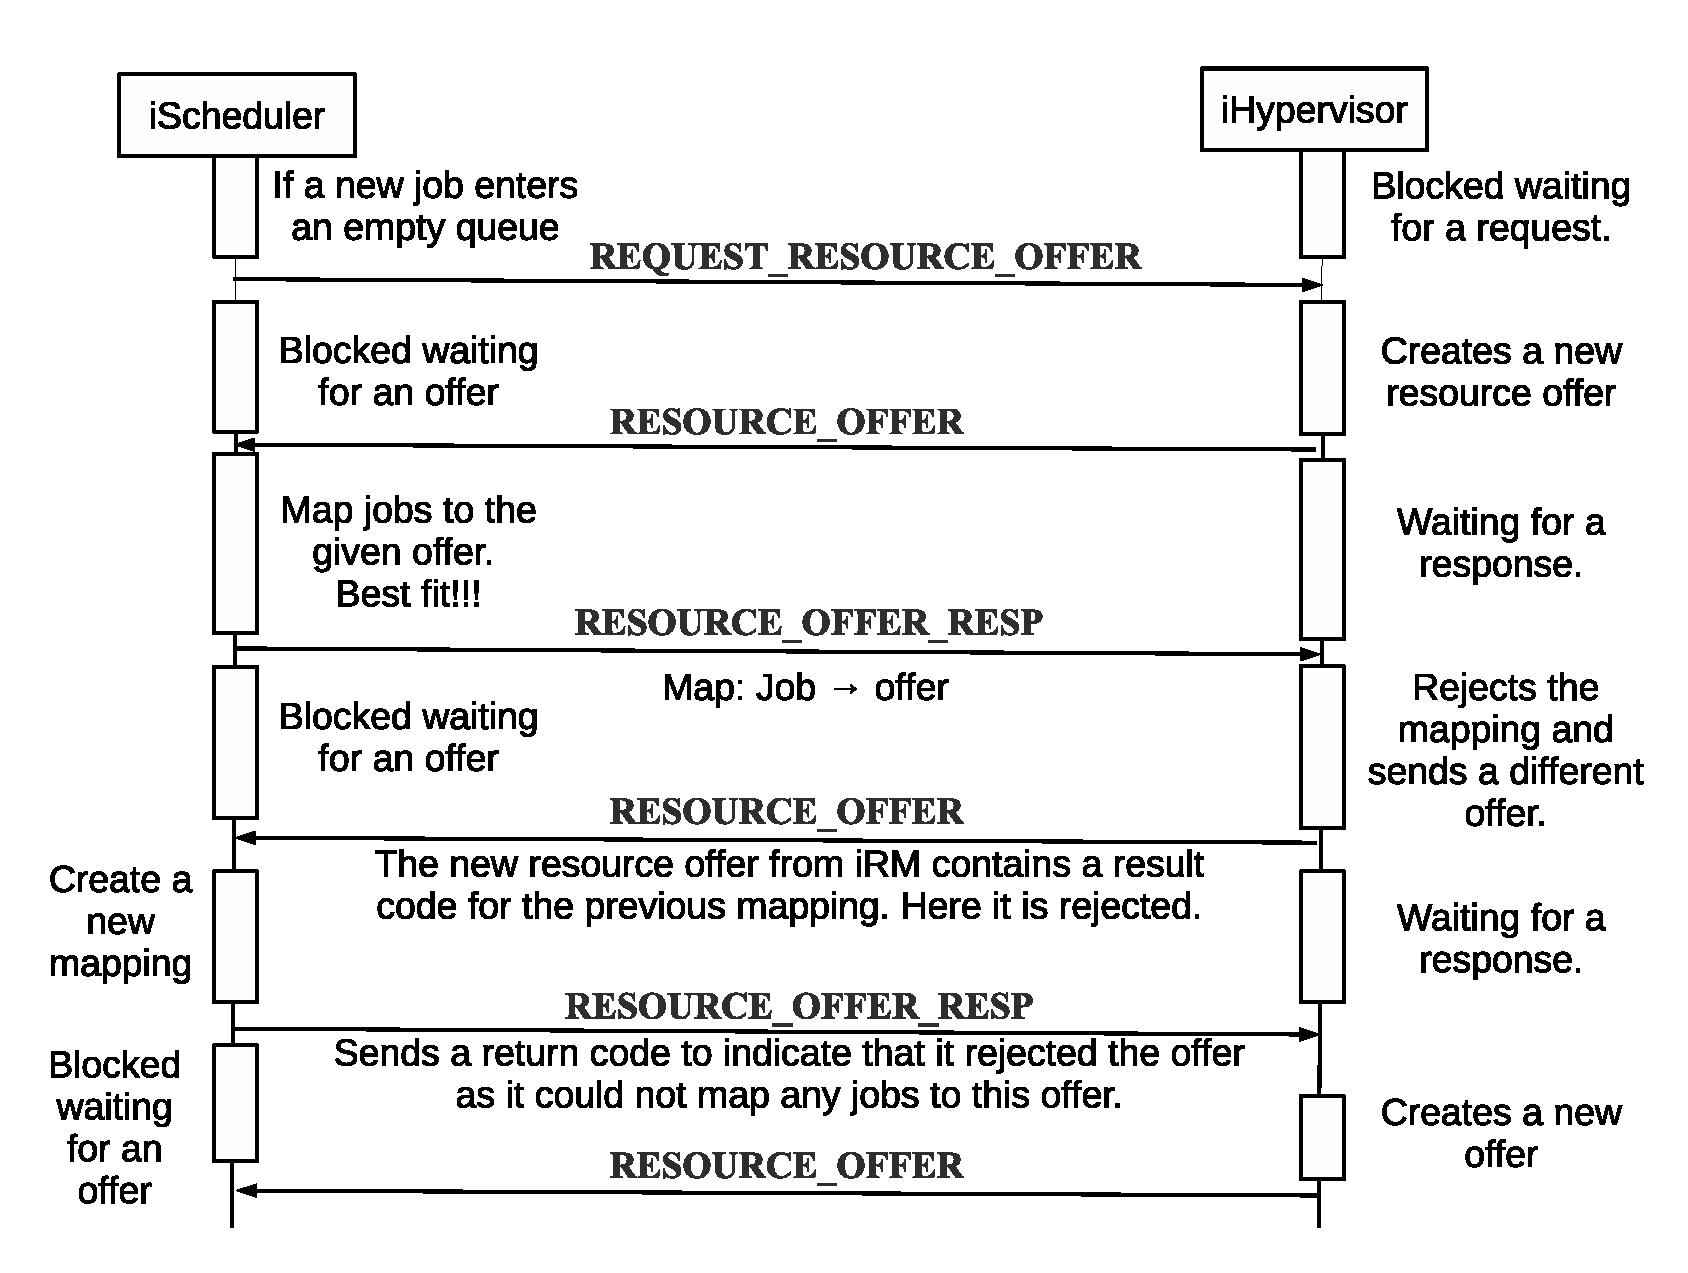
\includegraphics[width=1.0\textwidth, height=120mm]{./figures.eps}
\caption{Scenario 1}
\begin{itemize}
\item Above diagram illustrates a scenario where both iScheduler and iHpervisor are negotiating with each other. The scenario is continued in the next page. Figure[X] illustrates another scenario where negotiations may stop when job queue becomes empty and iHypevisor then will wait for a request from iScheduler for a resource offer that will happen when new jobs arrive.
\item iScheduler makes scheduling decisions at a coarser level of granularity which is nodes whereas iHypervisor does at the granularity of cores and sockets. Both will negotiate with each other till they reach an agreement.
\item It is an event based scheduling which means iScheduler makes a scheduling decision only when it is triggered by receiving a resource offer from iHypervisor. It is only at the start when there are no jobs in the queue and during the operations when the queue may become empty that the iScheduler will have to explicitly send a request message to iHypervisor for a resource offer otherwise at all other times scheduling is event based.
\end{itemize}
\label{fig:Seq1}
\end{figure}
\clearpage
\vspace{-0.25in}
\begin{figure}[!htbp]
\centering
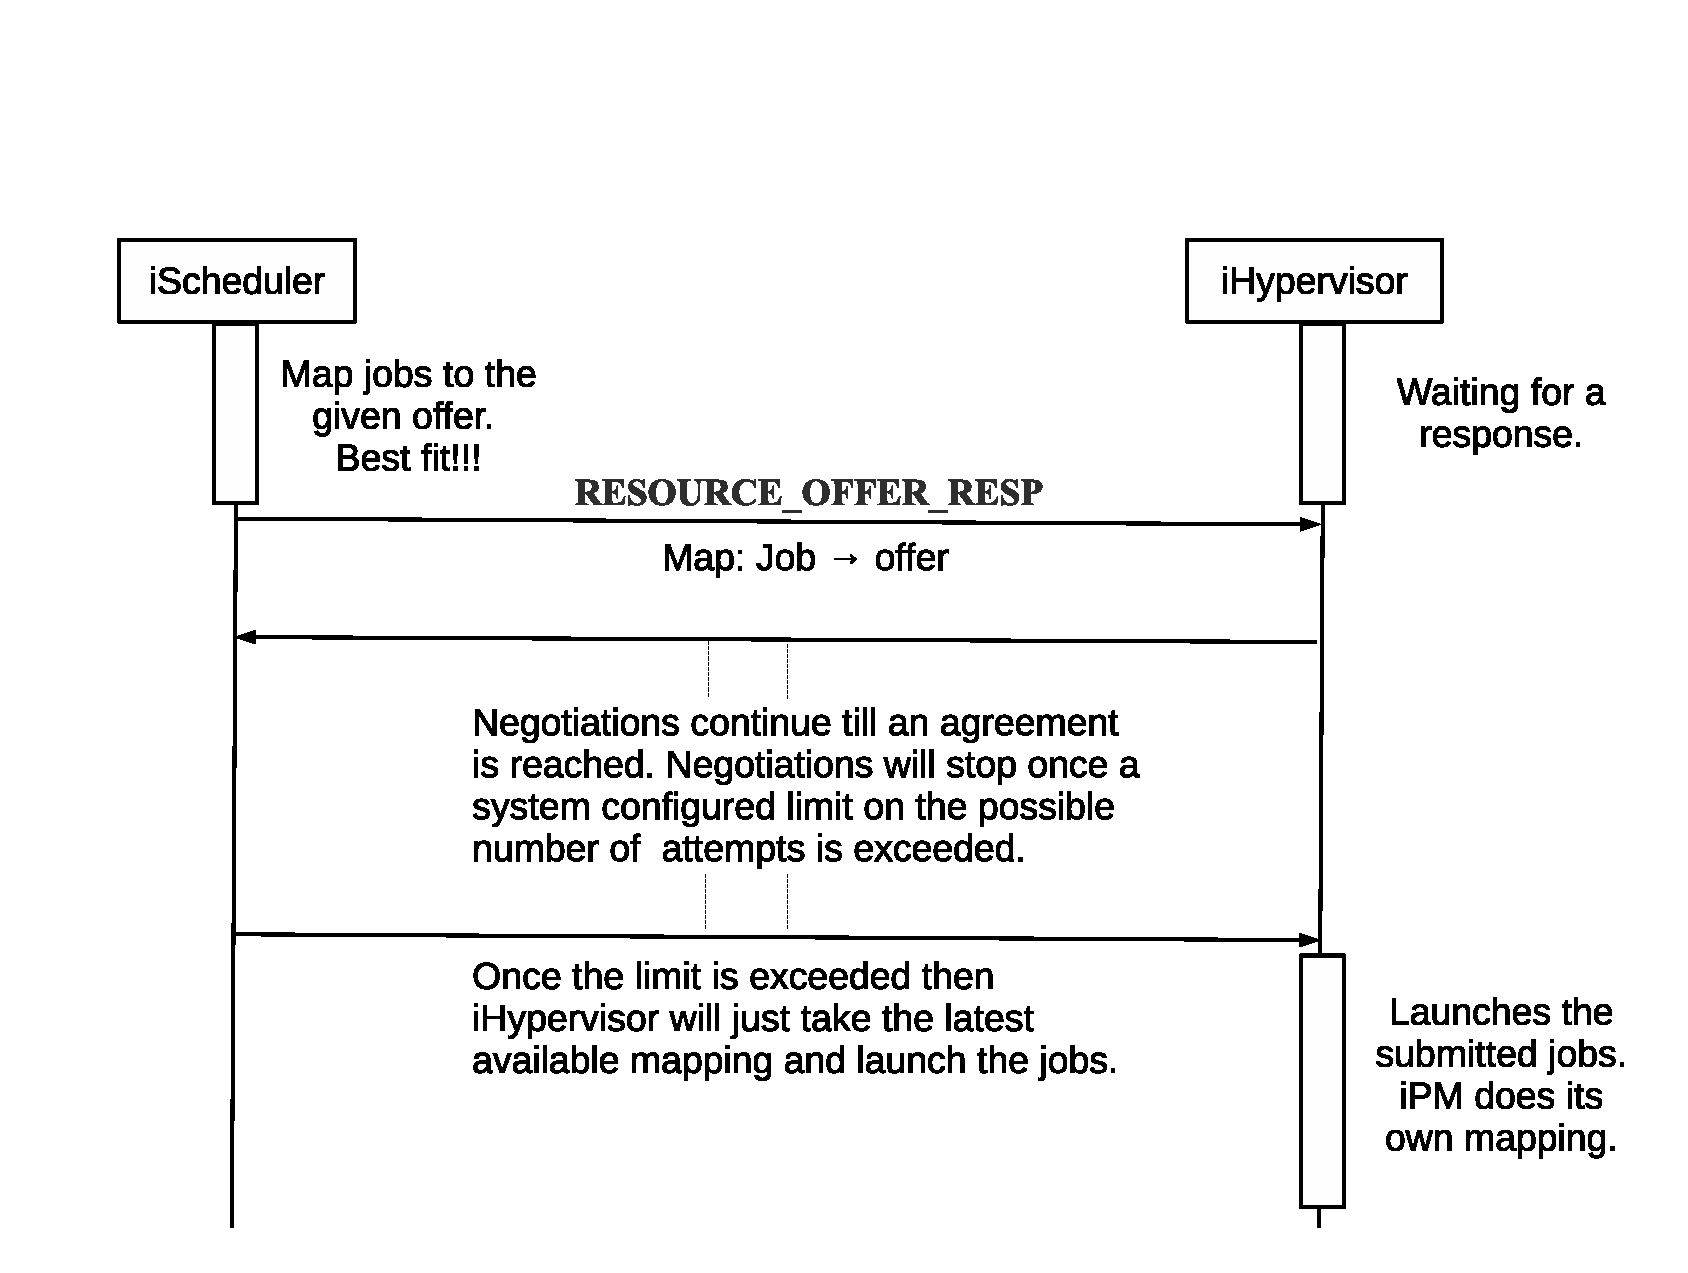
\includegraphics[width=0.9\textwidth, height=100mm]{./figures1.eps}
\caption{Scenario 1 contd.}
\label{fig:Seq1}
\vspace{0.25in}
%\end{figure}
%\begin{figure}[b]
\centering
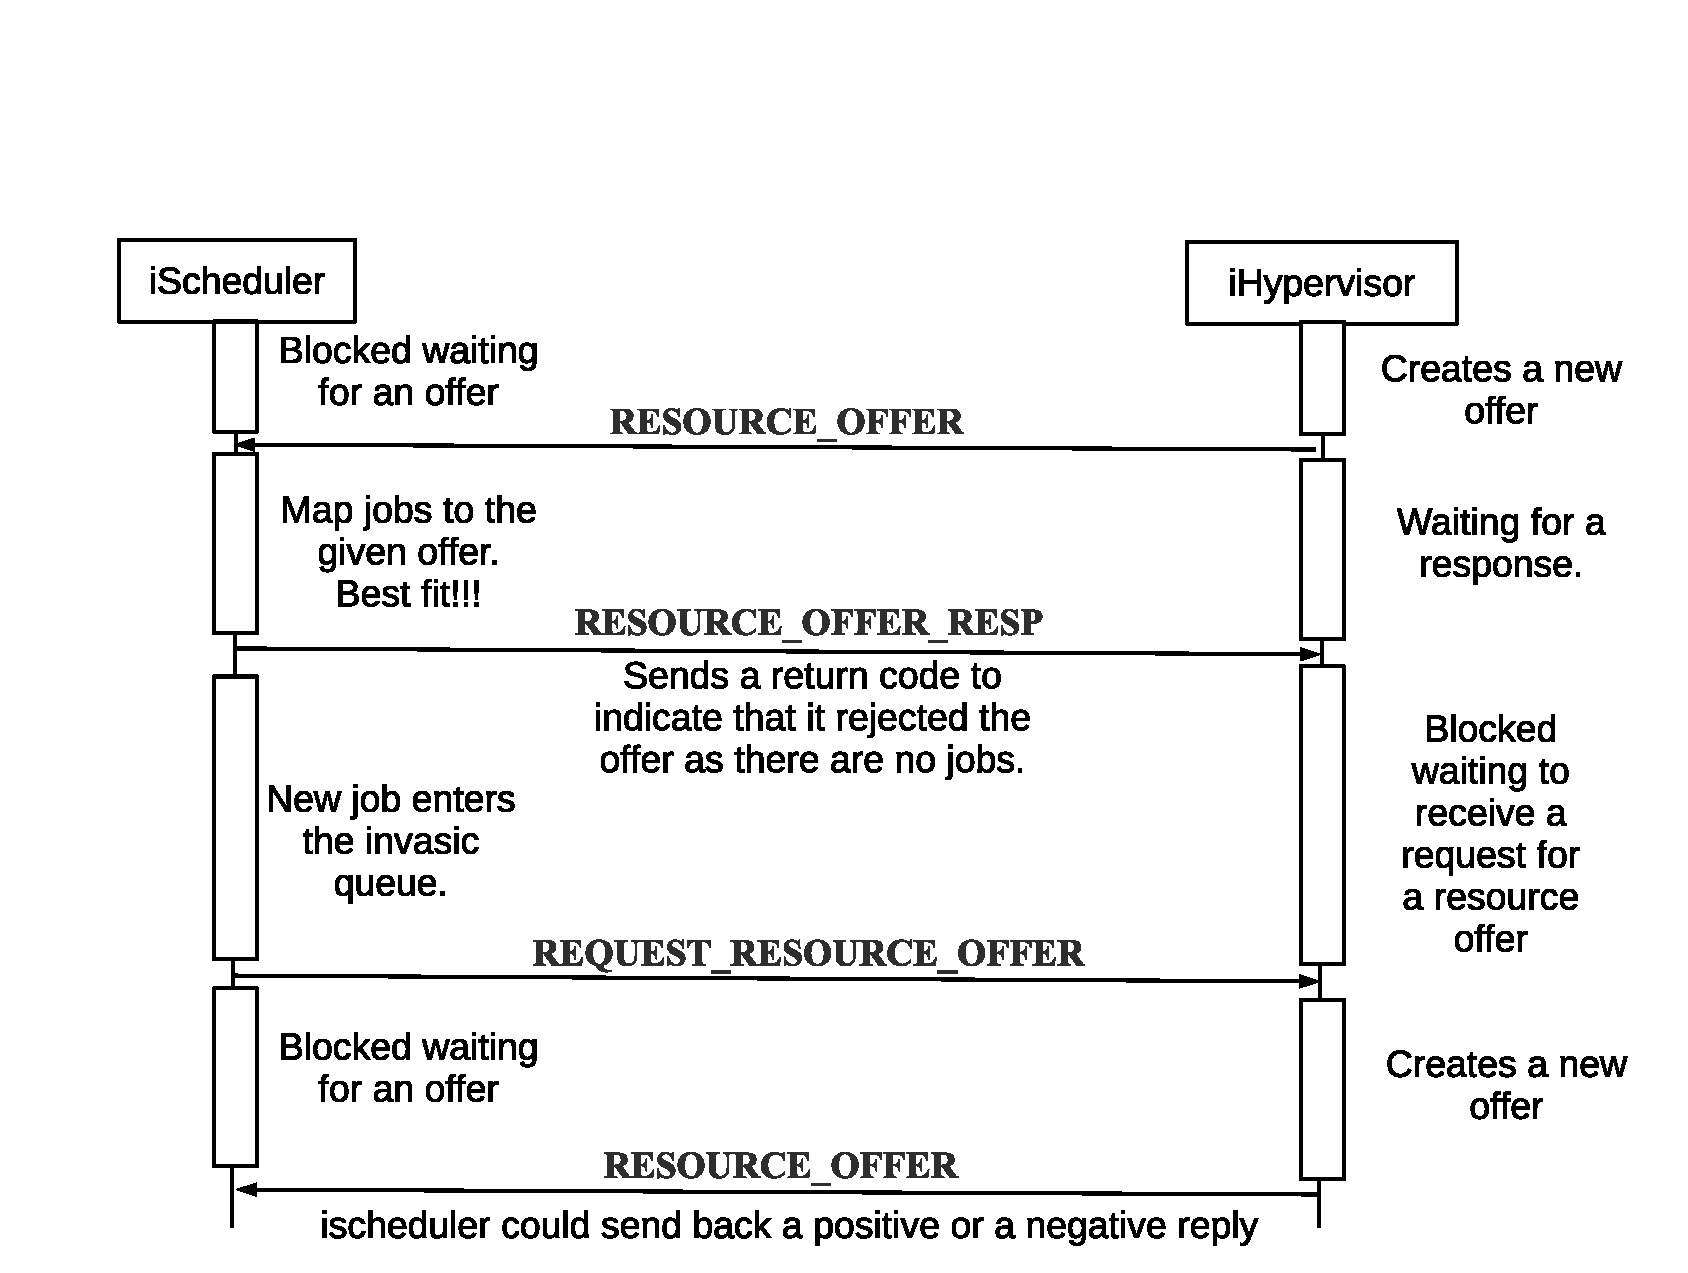
\includegraphics[width=0.9\textwidth, height=100mm]{./figures2.eps}
\caption{Scenario 2}
\label{fig:Seq2}
\end{figure}
\clearpage
\subsection{State Machine Diagrams}
This section focuses on iScheduler and a thread iRM\_AGENT that it spawns which is the one responsible for all the communication with the iHypervisor including spawning other agent threads for handling feedbacks and urgent jobs.
\vspace{10mm}
\begin{figure}[h]
\centering
\includegraphics[width=1.0\textwidth, height=150mm]{./"iRM Agent".eps}
\caption{iRM Agent}
\label{fig:Init}
\end{figure}
\begin{itemize}
\item Above diagram and the ones in the following pages illustrate state machine diagrams for few of the communication phases described earlier starting first with a general diagram of how the mulithreaded component iRM agent inside iScheduler starts up and shuts down.
\end{itemize}
\vspace{-20mm}
\begin{figure}[h]
\centering
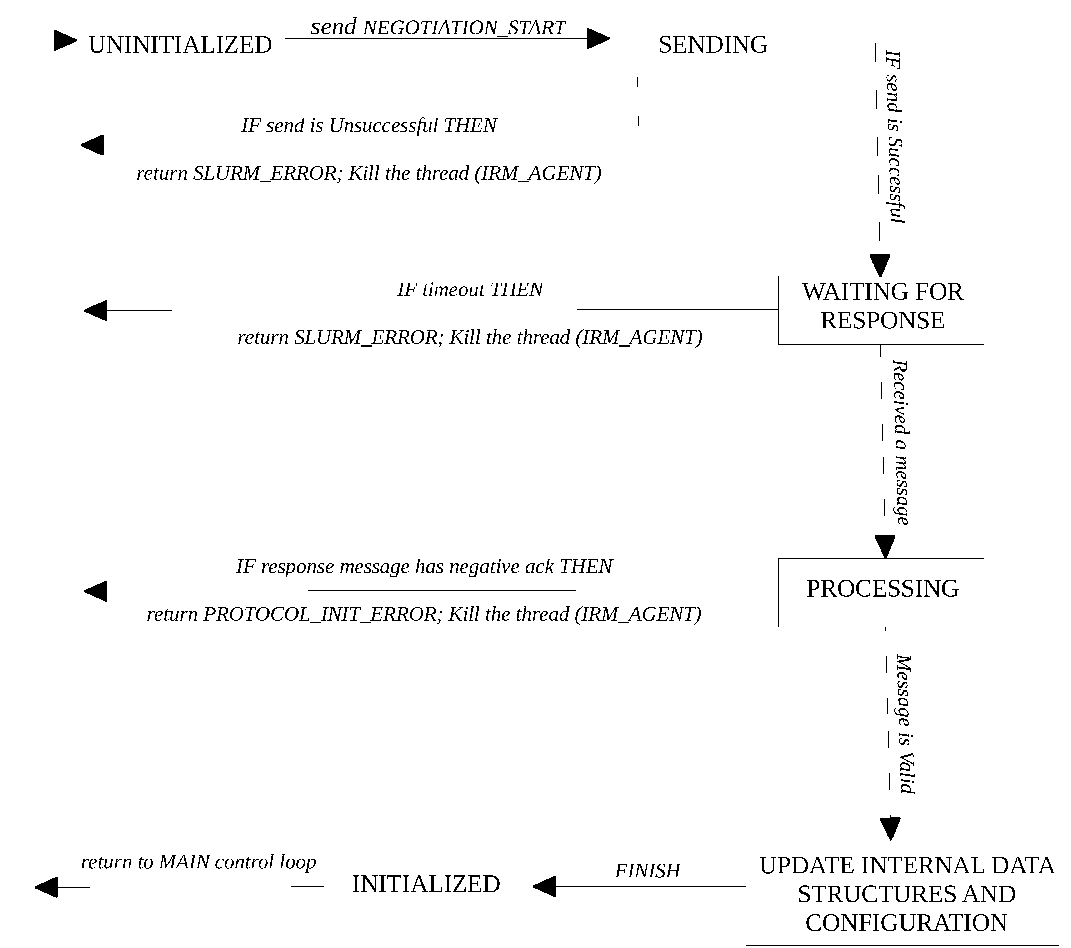
\includegraphics[width=0.9\textwidth, height=90mm]{./Init.eps}
\caption{Protocol Initialization}
\label{fig:Init}
\end{figure}
\vspace{5mm}
\begin{figure}[h]
\centering
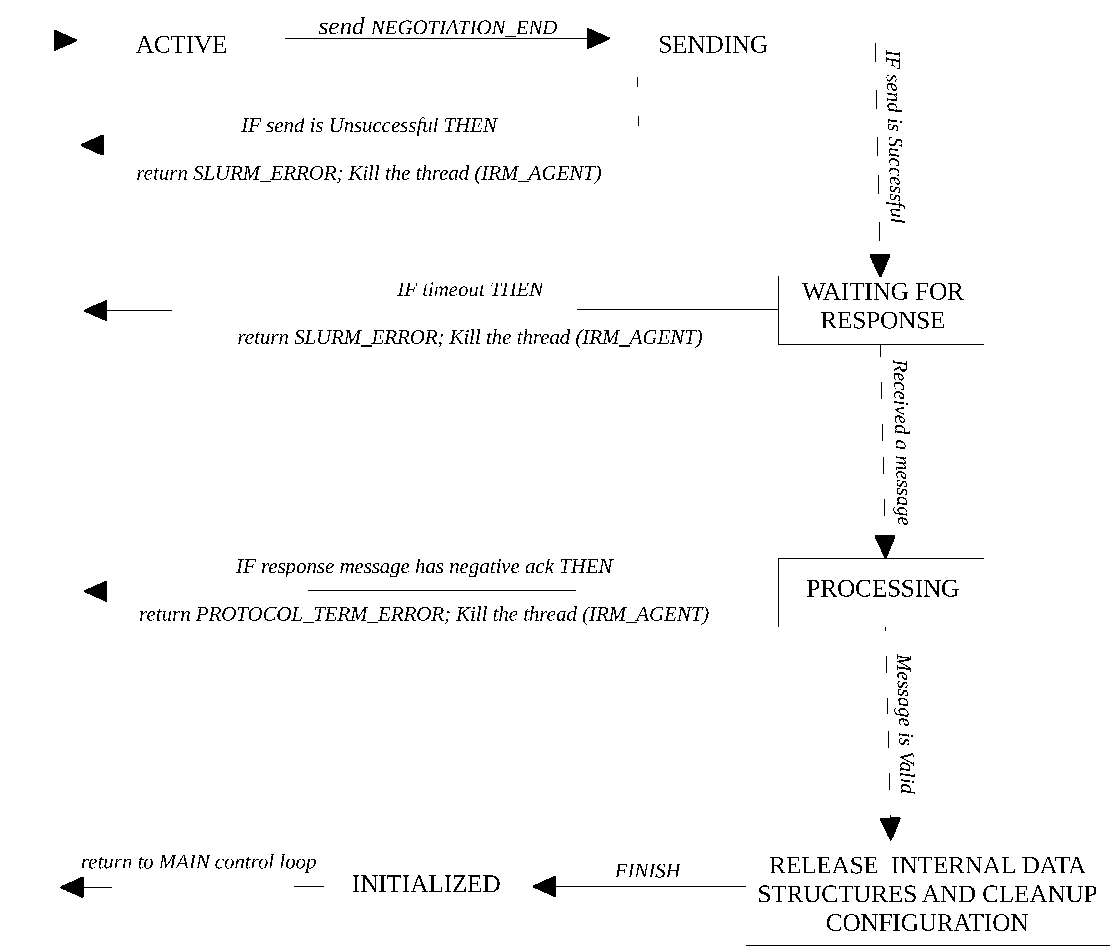
\includegraphics[width=0.9\textwidth, height=90mm]{./Term.eps}
\caption{Protocol Termination}
\label{fig:Term}
\end{figure}
\clearpage
\begin{figure}[h]
\centering
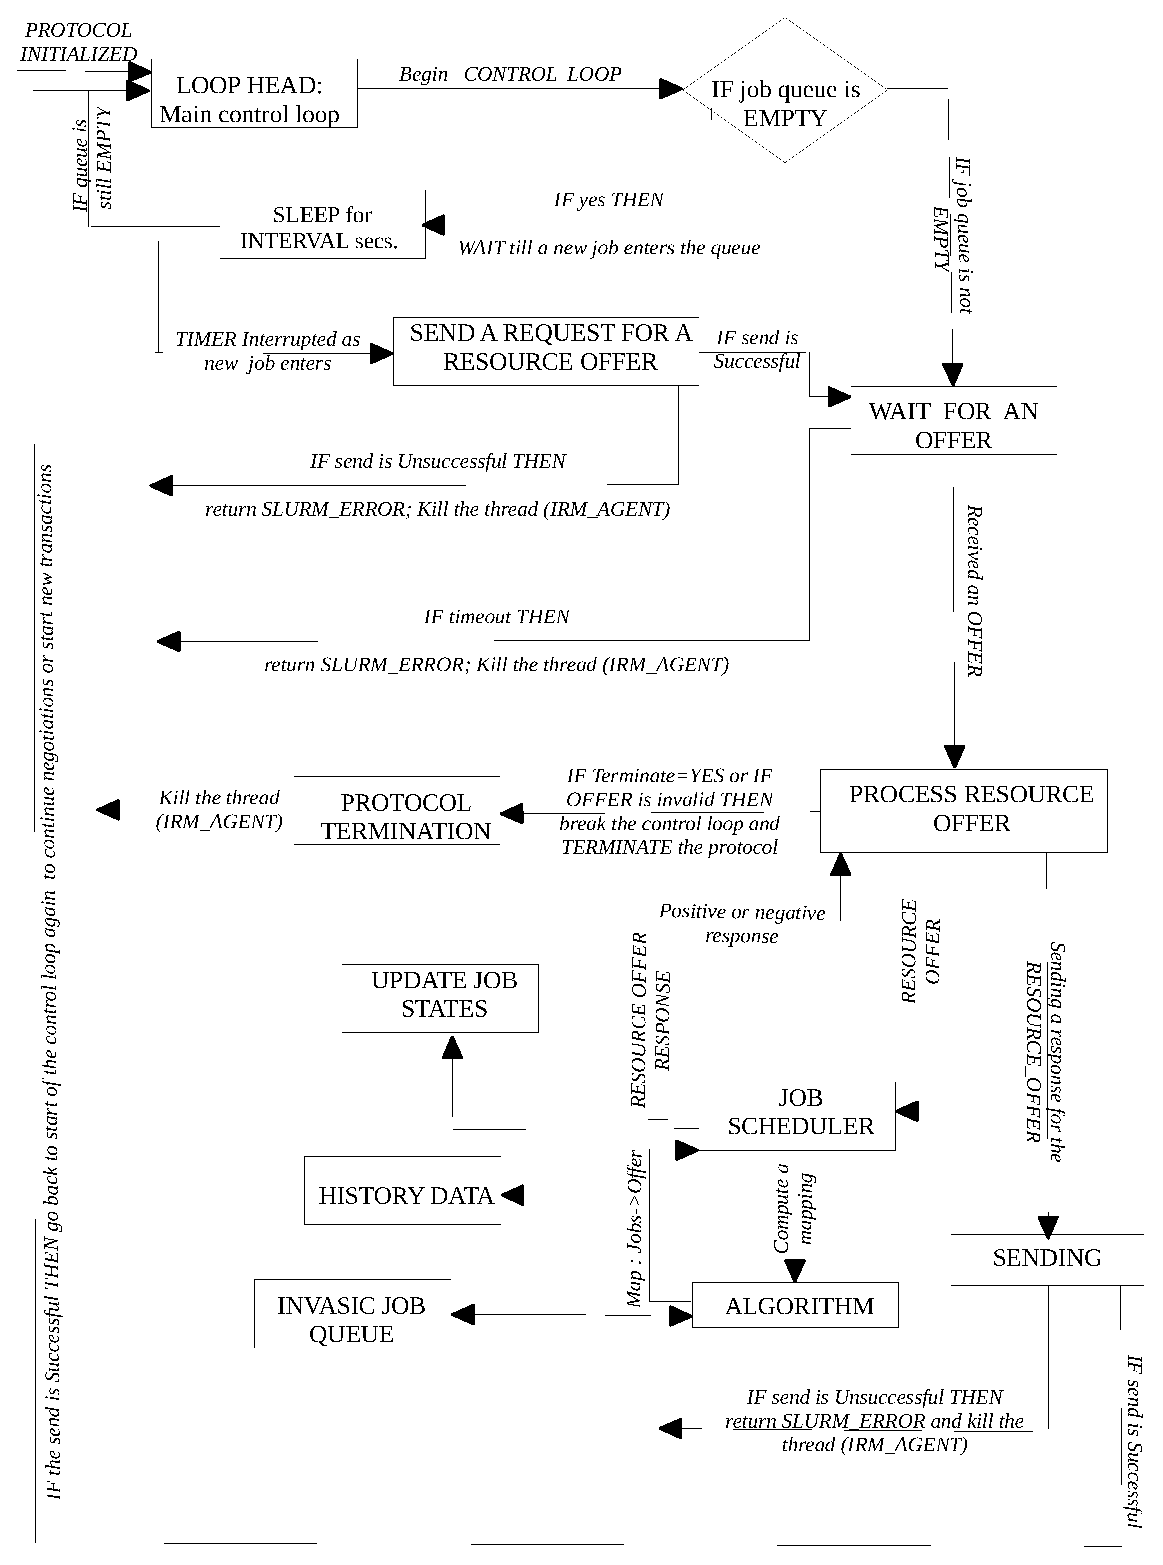
\includegraphics[width=1.0\textwidth, height=210mm]{./Negotiation.eps}
\caption{Negotiation}
\label{fig:Neg}
\end{figure}
\clearpage
\section{Conclusion}
The objective of this guided research was to implement a basic prototype to serve as a proof of concept for supporting a new programming paradigm called resource-aware programming in the domain of invasive computing for the upcoming exascale era. This will serve as a basic groundwork for further concrete implementations of scheduling algorithms, run time tuning of parallel applications, optimizing decision making at both the levels of iScheduler and iHypervisor through different approaches one of which could be machine learning. The basic communication infrastructure including the skeleton of protocol messages and the respective multithreaded communicating parties have been successfully implemented and tested for correctness.
%\begin{figure}[h]
%\centering
%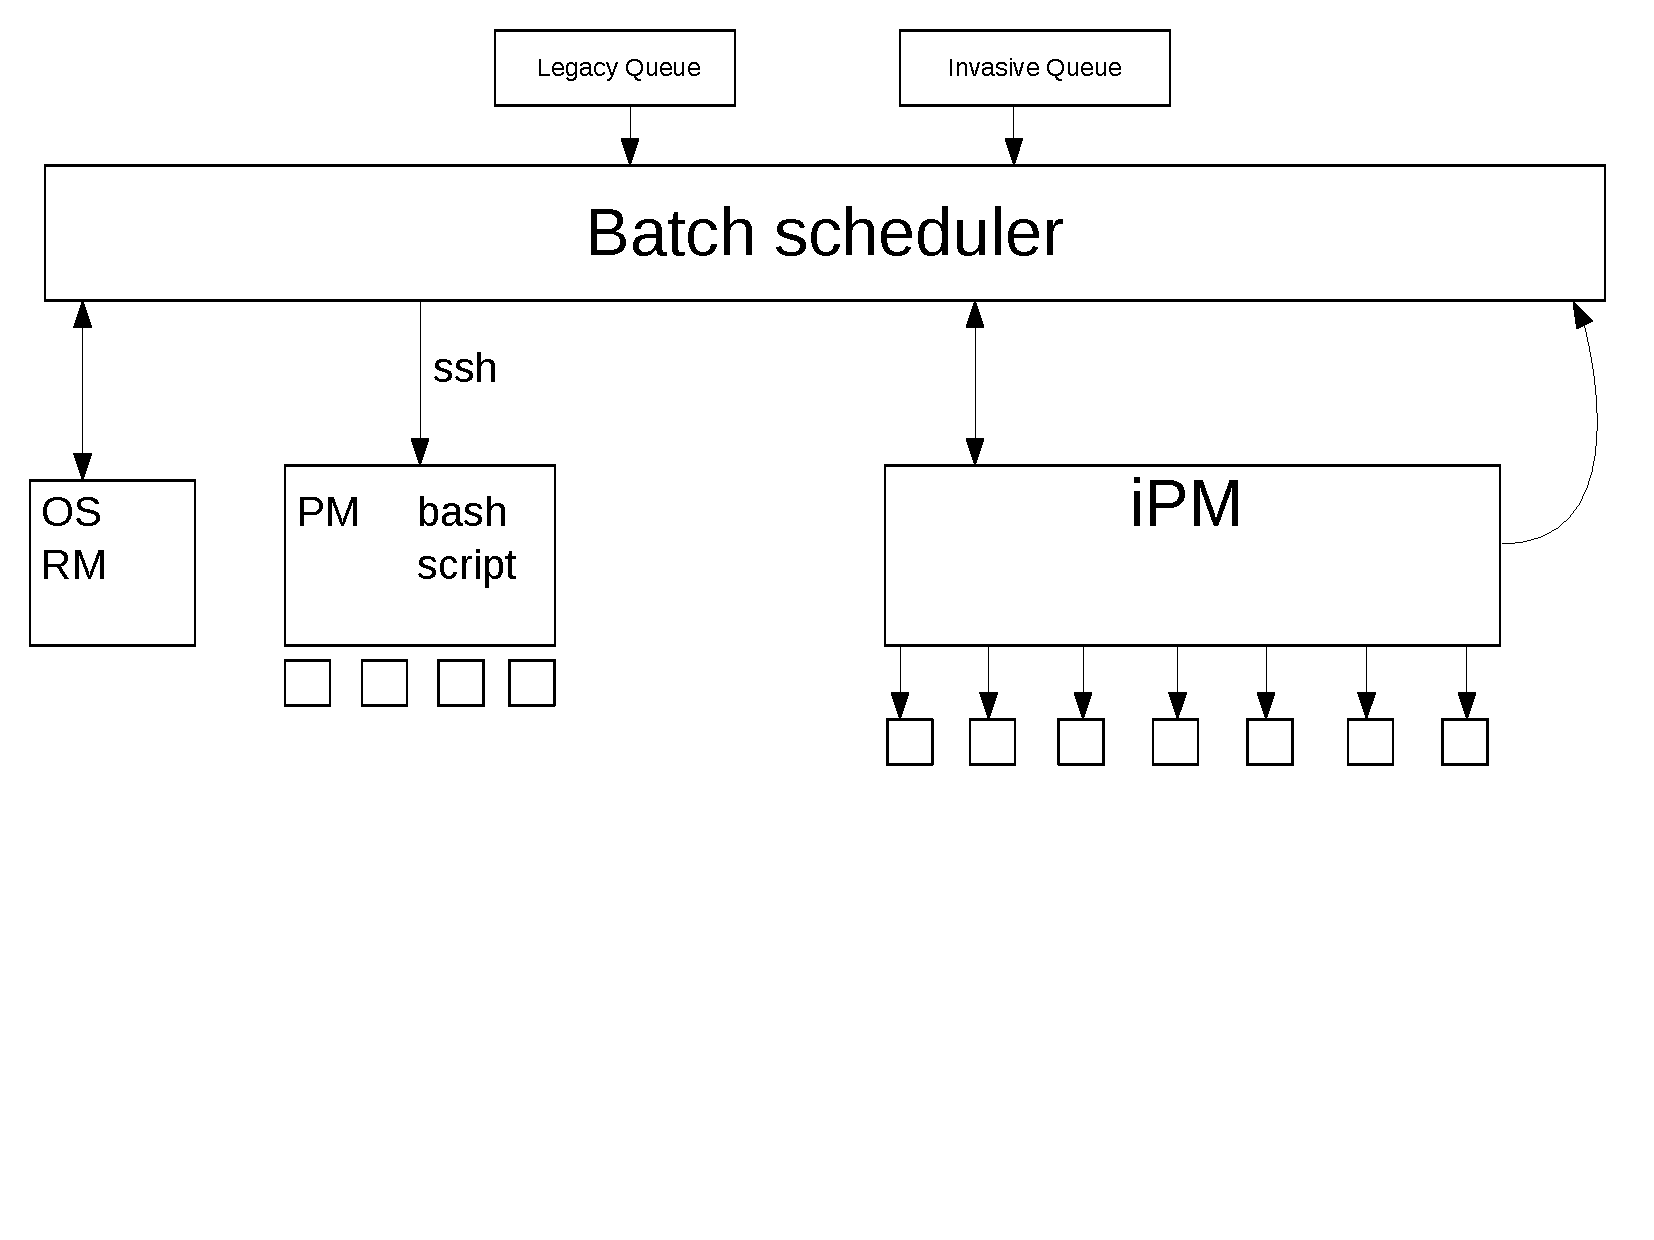
\includegraphics[width=0.65\textwidth, clip, trim=0mm 60mm 0mm 0mm]{data/architecture.pdf}
%\vspace{-0.15in}
%\caption{Invasive resource management architecture}
%\label{fig:arch}
%\end{figure}
%\nocite{fontaine,gao,poorzahedy2,tianze,leblanc,kuo,poorzahedy1,wen}
%\nocite{}

\bibliographystyle{unsrt}
% Literature sources are to be found in seminarpaper.bib
\bibliography{nishanth}

\end{document}
